\documentclass[a4paper,12pt,oneside]{article}

\usepackage{graphicx}
\usepackage{verbatim}
\usepackage{amsmath}
\usepackage[utf8]{inputenc}
\usepackage[colorlinks,bookmarks=false,linkcolor=blue,urlcolor=blue]{hyperref}
\usepackage{booktabs}

\paperheight=297mm
\paperwidth=210mm

\setlength{\textheight}{235mm}
\setlength{\topmargin}{-1.2cm}
%\setlength{\footskip}{5mm}
\setlength{\textwidth}{15cm}
\setlength{\oddsidemargin}{0.56cm}
\setlength{\evensidemargin}{0.56cm}

\pagestyle{plain}
\setcounter{secnumdepth}{2}


\newcommand{\mail}[1]{{\href{mailto:#1}{#1}}}
\newcommand{\ftplink}[1]{{\href{ftp://#1}{#1}}}


\begin{document}

\title{Chaos Déterministe}
\author{Laurent Rohrbasser \& Tim Tuuva}

\maketitle
\tableofcontents
\baselineskip=16pt
\parindent=15pt
\parskip=5pt

\begin{abstract}
%Résumé de l'expérience, on fait des tps sur le chaos, rappeler vite fait 
%dire le but de ces manips, qu'est ce qu'on veut?
\end{abstract}

\section{Introduction}
%expliqué les enjeux théoriques sur le chaos.
%domaine très théoriques
%peu de compréhension sur le sujet ( pourquoi???)

\newpage
\section{Dispositif}
%Description du dispositif expérimental
%Tim's duty
\subsection{Pendule inversé}

\subsubsection{Matériels}
%Oui c'est du copier coller je vais voir si je change ca
\begin{itemize}
	\item[--] Générateur de tension.
	\item[--] Générateur LD Series (A+D Products Bienne CH, EPFL TP Physique 466).
	\item[--] Pendule inversé (EPFL TP Physique 41).
	\item[--] Boitier ’Pendule chaotique’.
	\item[--] Boitier SensorCassy (Leybold Didactic Gmbh).
	\item[--] Voltmètre.
\end{itemize}

\subsubsection{Schéma}

\begin{figure}[h!]
  \begin{center}
  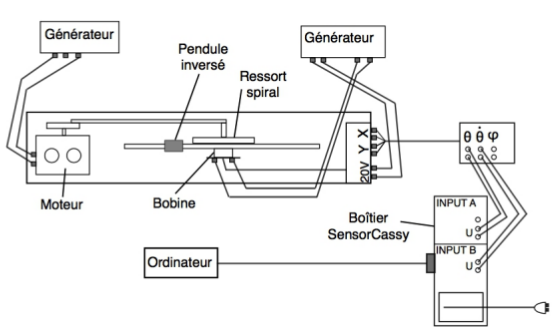
\includegraphics[width=0.5\linewidth,angle=0]{./figures/pendule_inverse.png}
  \caption{Schéma du dispositif du pendule inversé pour le TP sur le chaos déterministe.} \label{fig:pendule1}
  \end{center}
\end{figure}

\subsubsection{Procédure}

%TODO PEAUFINER
Le pendule inversé est muni d'un potentiomètre, alimenté par un premier générateur, dont la position angulaire correspond à $\theta$ et sa vitesse angulaire à $\dot{theta}$. Celui ci est relié au boitier pendule chaotique.
Le dispositif mesure, grâce au boitier SensorCassy, les valeurs de $\theta$ et $\dot{\theta}$,
permettant de tracer l'espace de phase du pendule inversé.
Un moteur alimenté par un deuxième générateur, peut provoquer une perturbation sur l'axe du ressort, ce qui engendre des effets de résonnance ou de mouvement chaotique. Il est aussi possible d'utiliser un frein electromagnétique pour réaliser des perturbations.

L'objectif est donc de trouvé une tension d'alimentation du moteur, tel que la fréquence d'excitation provoque des mouvement chaotique du ressort, obtenu grâce à l'analyse des diagramme de phase.

Le moteur est alimenté tel que: $U_{alimentation}=2-5$ [V].
La sonde du pendule est alimenté tel que: $U_{alimentation}=10-20$ [V].
\subsection{Moteur dipolaire}

\subsubsection{Materiels}
\begin{itemize}
	\item[--] Générateur de fonctions: Wavetek, IPE 241-07/03.
	\item[--] Générateur d’impulsions: EPFL, IPE 242 - 07/03.
	\item[--] Oscilloscope: Hewlett Packard, HP 54600A.
	\item[--] Sonde de Hall : Bell 620 Gaussmeter, IPE 240 - 07/03.
	\item[--] Amplificateur C.C. : EPFL.
	\item[--] Moteur bipolaire : EPFL.
\end{itemize}

\subsubsection{Schéma}
\begin{figure}[h!]
  \begin{center}
  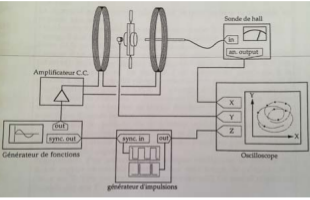
\includegraphics[width=0.8\linewidth,angle=0]{./figures/moteur1.png}
  \caption{} \label{fig:}
  \end{center}
\end{figure}


\subsubsection{Procédure}

Un générateur de fonction permet d'envoier un signal triangulaire au
 bornes d'un aimant d'Helmotz, qui va provoquer une perturbation du
 moteur dipolaire, forcant sa redirection momentanément. Sur l'oscilloscope, l'entrée X est reliée à une
 sonde de Hall mesurant l'angle $\theta$ du moteur dipolaire via la variation du champ magnétique,
 l'entrée Y est reliée à un électroaimant dont on
 mesure la variation de courant, induit par le champ magnétique
 variant du moteur dipolaire, représentant $\dot{\theta}$. La fonction trigger est utilisé grâce
 à une sorti sync. sur le générateur de fonction.

En utilise la fonction "XY display" de l'oscilloscope, il est possible de voir le diagramme de phase du moteur dipolaire sous l'influence d'un champ magnétique oscillant  une certaine fréquence.

Il faut trouvé des fréquence d'excitation, tel que le mouvement soit 1 fois périodique, 2 fois périodique ou chaotique. Ceci est possible en utilisant le trigger et en observant le nombre de point distingue tracé sur le diagramme de phase.

Par le suite, une schéma de bifurcation est réalisable en applicant la sorti du générateur de fonction directement sur l'entrée X de l'oscilloscope. Ceci représente le diagramme ($\theta$,$XXX$).%TODO COMPLETER XXX

\section{Résultats}
%Exposition des graphes avec les légendes et un peu de texte explicatifs sur comment on les a obtenus.

\subsection{Pnedule inversé}

\begin{figure}[h!]
  \begin{center}
  \includegraphics[width=0.8\linewidth,angle=0]{./figures/1_1_001_lab.pdf}
  \caption{Illustration de la difficulté à obtenir une symétrie du pendule inversé tel qu'il y a deux positions d'équilibre.} \label{fig:1_1_001_lab}
  \end{center}
\end{figure}

\begin{figure}[h!]
  \begin{center}
  \includegraphics[width=0.8\linewidth,angle=0]{./figures/1_1_008_lab.pdf}
  \caption{Tentative de rééquilibrage du pendule, la position de repos du pendule est passé de droite à gauche, cependant la présence d'une double position d'équilibre n'est pas encore effective.} \label{fig:1_1_008_lab}
  \end{center}
\end{figure}

\begin{figure}[h!]
  \begin{center}
  \includegraphics[width=0.8\linewidth,angle=0]{./figures/1_2_U_10_95_lab.pdf}
  \caption{Illustration de l'inutilité d'appliquer une fréquence trop élevé au pendule avec $\omega\approx XXX$.} \label{fig:1_2_U_10_95_lab}
  \end{center}
\end{figure}

\begin{figure}[h!]
  \begin{center}
  \includegraphics[width=0.8\linewidth,angle=0]{./figures/1_2_U_2_41_lab.pdf}
  \caption{$\omega \approx$} \label{fig:1_2_U_2_41_lab}
  \end{center}
\end{figure}

\begin{figure}[h!]
  \begin{center}
  \includegraphics[width=0.8\linewidth,angle=0]{./figures/1_2_U_3_02_lab.pdf}
  \caption{Présence d'un attracteur aux abords de la position droite du pendule, $\omega \approx$} \label{fig:1_2_U_3_02_lab}
  \end{center}
\end{figure}

\begin{figure}[h!]
  \begin{center}
  \includegraphics[width=0.8\linewidth,angle=0]{./figures/1_2_U_3_44_lab.pdf}
  \caption{Illustration de la convergence vers une position d'équilibre du pendule, malgré une perturbation crée par le moteur, avec $\omega \approx$} \label{fig:1_2_U_3_44_lab}
  \end{center}
\end{figure}

\begin{figure}[h!]
  \begin{center}
  \includegraphics[width=0.8\linewidth,angle=0]{./figures/1_2_U_4_54_lab.pdf}
  \caption{Illustration de la convergence vers une position d'équilibre du pendule, malgré une perturbation crée par le moteur, avec $\omega \approx$Illustration de la convergence vers une position d'équilibre du pendule, malgré une perturbation crée par le moteur, avec $\omega \approx$} \label{fig:1_2_U_4_54_lab}
  \end{center}
\end{figure}

\begin{figure}[h!]
  \begin{center}
  \includegraphics[width=0.8\linewidth,angle=0]{./figures/1_2_U_4_97_theta__FREIN_PAS_FREIN_lab.pdf}
  \caption{Passage d'un mode périodique à un mode chaotique par application d'un frein électromagnétique avec $\omega \approx XXX$} \label{fig:1_2_U_4_97_theta__FREIN_PAS_FREIN_lab}
  \end{center}
\end{figure}

\begin{figure}[h!]
  \begin{center}
  \includegraphics[width=0.8\linewidth,angle=0]{./figures/1_2_U_5_63_lab.pdf}
  \caption{Problème de symétrie} \label{fig:1_2_U_5_63_lab}
  \end{center}
\end{figure}

\begin{figure}[h!]
  \begin{center}
  \includegraphics[width=0.8\linewidth,angle=0]{./figures/1_3_U_5_01_lab.pdf}
  \caption{Illustration de la différence de mouvement selon différentes conditions initiales avec $\omega\approx$ fixé. Avec une plus grande énergie initiale l'aspect chaotique disparait.} \label{fig:1_3_U_5_01_lab}
  \end{center}
\end{figure}
\section{Discussion}%le plus important

\subsection{Interprétation}
%Qu'est ce que les résultats nous permettent de conclure?
%Est ce que cela nous aide pour nôtre but?

\subsection{Discussions}
%Validité de nos résultats
%S'il y a des erreurs, d'ou viennent elle!
%Avons nous atteind les buts du TP?
\section{Conclusion}

%Résumer du rapport
%Ouverture





%Reference
\begin{thebibliography}{99}
\end{thebibliography}

\end{document}
